\documentclass[11pt]{ctexart}

\usepackage[a4paper,margin=1in]{geometry}
\usepackage{amsmath,amssymb}
\usepackage{booktabs}
\usepackage{array}
\usepackage{enumitem}
\usepackage{graphicx}
\usepackage{caption}
\usepackage{float}
\usepackage{xcolor}
\usepackage{hyperref}
\usepackage{fancyhdr}

\hypersetup{
  colorlinks=true,
  linkcolor=black,
  citecolor=black,
  urlcolor=blue
}

\definecolor{agenblue}{RGB}{27,80,156}
\definecolor{agengray}{RGB}{82,88,101}

\setlength{\parindent}{2em}
\setlength{\parskip}{0.35em}
\setlength{\headheight}{14pt}
\setlist[itemize]{leftmargin=2em,itemsep=0.2em,topsep=0.25em}
\setlist[enumerate]{leftmargin=2em,itemsep=0.2em,topsep=0.25em}
\captionsetup{font=small,labelfont=bf}
\allowdisplaybreaks
\sloppy

\pagestyle{fancy}
\fancyhf{}
\lhead{\textcolor{agengray}{AgenQA Project Preview}}
\rhead{\textcolor{agengray}{Scientific Reasoning QA Synthesis}}
\cfoot{\thepage}
\renewcommand{\headrulewidth}{0.4pt}

\newcommand{\agenqatitle}{AgenQA: An Agentic Harness for Synthesizing Challenging Reasoning QA via Growth and Folding of Step-Verifiable Dependency Chains}
\newcommand{\tightparagraph}[1]{\vspace{0.4em}\noindent\textbf{#1}}

\begin{document}

\begin{center}
{\LARGE \bfseries \agenqatitle \par}
\vspace{0.8em}
{\large 冯亮 \par}
\vspace{0.25em}
{\small Project preview for AI research / RA hiring context \par}
\vspace{0.8em}
{\small 2026 年 5 月 \par}
\end{center}

\begin{abstract}
AgenQA 研究如何合成具有挑战性的 scientific reasoning QA 数据，同时不失去可验证性。它不把 QA generation 视为一次性生成最终难题，而是先构造一条 step-verifiable Chain-of-KQA，再通过 Path-Fold 隐藏中间事实，形成更难的 solver-facing Path View；与此同时，局部 Edge View 保留了 step-level correctness control 所需的可见支撑。系统上，AgenQA 将生成过程组织为 Director--Operator--Evaluator loop：Director 选择 init / extend / revise / finish，Operators 修改显式 chain state，Evaluator 通过 solvers、consensus 和 contract signals 给出在线反馈。阶段性评测显示，AgenQA 生成的 Path View 题目能形成有效的 model-discrimination signal：在一组 SOTA solver 评测中整体准确率为 84.18\%，诊断子集准确率为 51.77\%；在 Qwen-family 梯度评测中，准确率随模型规模从 48.00\% 提升到 66.86\%。这些结果表明，AgenQA 的核心价值不是简单生成更长题面，而是把局部可检查的 dependency growth 转化为全局可挑战、可诊断的 benchmark items。
\end{abstract}

\section{Introduction}

面向 challenging reasoning QA 的高质量数据不只服务于 benchmark，它同时是评估和改进大语言模型的共同数据基底。它可以被实例化为 benchmark、supervised fine-tuning examples、reinforcement-learning tasks，或者 post-training 中的 curriculum data。

随着模型具备更强的指令遵循能力和更长的 inference-time reasoning 能力，如果每条答案背后的推理结构缺失，扁平 question-answer data 的诊断和训练价值都会下降。最终答案可以告诉我们模型是否答对，却很难解释成功来自稳健的多步推理、浅层模式匹配、幸运猜测，还是训练阶段已经见过相似实例。

与此同时，人工构造新鲜且具有挑战性的 reasoning questions 速度慢、成本高，也难以规模化。这推动了 synthetic QA data、自动 benchmark 构建以及 agent-assisted problem generation 等方向的发展。

\subsection{The Correctness--Difficulty Tension}

合成高质量 challenging reasoning QA 并不只是让强模型生成更难的问题。核心困难在于：既要得到真正困难的问题，又要让构造过程保持可检查。

One-shot generation 往往首先失败在 difficulty 这一侧。强模型被要求出难题时，常常会生成仍落在自身解题分布内的问题，因此未必能挑战同级别 solver。继续用同一个 one-shot 过程制造表面难度时，又容易引入隐含假设、题面不完整、答案不稳定或答案等价性不可验证等问题。

反过来，如果题目被拆成小而完全暴露的步骤，每个局部步骤会更容易验证，但也可能过于简单，无法挑战强 solver。

\subsection{The AgenQA Object: Local Edges and Folded Paths}

AgenQA 围绕 step-level correctness control 与 global difficulty amplification 的显式分离来组织 challenging reasoning QA synthesis。它将 reasoning-QA synthesis 从一次性生成 final question，转化为先 progressive construction 一条 step-verifiable \textbf{Chain-of-KQA}，再通过 \textbf{Path-Fold} 隐藏中间推导步骤，把这条 chain 转化为 challenging final question。

这里的 \textbf{Edge} 和 \textbf{Path} 采用 graph sense：Edge 表示一个局部 dependency transition，Path 表示由这些 transitions 组成的多步 dependency route。每个 KQA transition 都绑定 local known state、question、answer-equivalent key fact 和 dependency certificate。

在 Edge View 中，solver 会获得推出下一个 fact 所需的局部上下文，因此该 transition 更容易被验证和审计。在 Path View 中，Path-Fold 会隐藏中间推导步骤，迫使 solver 从初始 premises 到最终答案重构整条 route。因此，局部 transitions 可以保持在强模型可验证的范围内，而折叠后的 path 可以变成全局困难问题。

\subsection{Agentic Synthesis Harness}

这种形式化改变了 agent 在 QA generation 中的角色。AgenQA 并不把 agent 当成黑箱式出题者，而是让 agent 在显式 reasoning state 上操作。整个 synthesis process 被实现为一个受控 state-transition loop：

\begin{itemize}
  \item \textbf{Director} 读取当前 chain state、可选 operations 和 evaluator feedback；
  \item \textbf{Operators} 通过 initialization、extension 或 revision 修改 Chain-of-KQA state；
  \item \textbf{Edge/Path views} 在不同 visibility 条件下把状态暴露给 solvers；
  \item \textbf{Evaluator} 通过 solvers 和 consensus 检查这些 views，并返回 acceptance 与 repair signals。
\end{itemize}

在这个循环中，quality control 不是生成之后附加的 post-hoc filter，而是 generation process 本身的一部分。

\section{Background and Motivation}

\subsection{Synthetic Reasoning Data Background}

面向科学与复杂推理的 synthetic data 并不只是“生成更多题目”。MegaScience~\cite{fan2025megascience} 等科学后训练数据工作表明，数据的答案可靠性、去污染、长度控制、领域覆盖和配方都会影响下游模型是否真正学到推理能力。Data Darwinism~\cite{qin2026datadarwinism} 进一步从数据加工层级提醒我们，高价值数据需要从原始文本或简单问答转化为更可学习、更可验证、更接近任务环境的对象。

由此看，challenging reasoning QA synthesis 的问题不是规模本身，而是如何构造一种既能承载复杂推理，又能被检查、筛选和复用的数据对象。

\subsection{Synthesis Paradigms}

已有 synthetic reasoning-data 方法可以按生成机制分为几类：seed 或 evolution-based methods 从已有题目出发改写或提升复杂度，如 Self-Instruct、WizardMath、MetaMath 和 Auto Evol-Instruct~\cite{wang2023selfinstruct,luo2025wizardmath,yu2024metamath,zeng2024autoevolinstruct}；composition-based methods 将已有可解题目或 prompts 组合成更长任务，如 R-HORIZON 和 Composition-RL~\cite{lu2025rhorizon,xu2026compositionrl}；bottom-up verifiable-subtask methods 从可检查的子任务构造困难题，如 CHASE~\cite{patel2025chase}；agentic benchmark pipelines 将 benchmark creation 拆成 planning、generation、verification 和 evaluation，如 BenchAgents~\cite{butt2025benchagents}；agentic proposing methods 将 problem synthesis 组织为 sequential decision process~\cite{jiao2026agenticproposing}。

这些范式共同说明，合成高价值推理数据已经从一次性文本生成，转向受控构造过程。

\subsection{Dependency Paths as Control Objects}

已有范式往往把“如何提高 difficulty”和“如何维持 correctness”耦合在一起。Direct final-QA generation 或 evolution 通常通过更复杂的题面来追求难度，但这会带来双重失败模式：强模型被要求生成难题时，仍可能产出落在自身解题分布内的问题，所以表面难度不一定转化为 solver difficulty；如果继续提高表面难度，又容易引入隐含条件、题面不自足、答案不稳定或不可解实例。

Composition-based methods 试图通过放大 long-horizon structure 来缓解这一点。但如果 composition 发生在 individual items 生成之后，dependency failures 很难在 synthesis 过程中被定位和修复。CHASE 这类 bottom-up methods 更接近我们的目标，因为它把 verifiable subtasks 纳入 difficult-problem construction；但对 AgenQA 来说，关键还不只是“有子任务”，而是 intermediate dependencies 能否被维护为一个统一 state：它要能持续生长、能 step by step 地检查，并且之后能转化为 hard solver-facing problem。

因此，hard-QA synthesis 需要一个不同的 control object：从初始 known context 连接到最终答案的 dependency path。AgenQA 不把复杂推理结构只当作 latent problem quality、post-hoc composition structure 或 iterative generation 的副产品，而是将其 materialized 为 persistent path state。

Path-Fold 的动机正来自这个缺口：生成侧应保留 dependency path 用于检查和修复，而 solver-facing problem 应折叠或隐藏中间结论，使难度来自对一条可靠路径的重构，而不是不可验证的一次性复杂化。

\section{Method: The AgenQA Framework}

AgenQA 不把 challenging reasoning-QA synthesis 视为一次性生成最终难题，而是先构造一条 step-verifiable reasoning chain，再通过 Path-Fold 隐藏中间推理步骤，形成全局更困难的问题。

\begin{figure}[H]
  \centering
  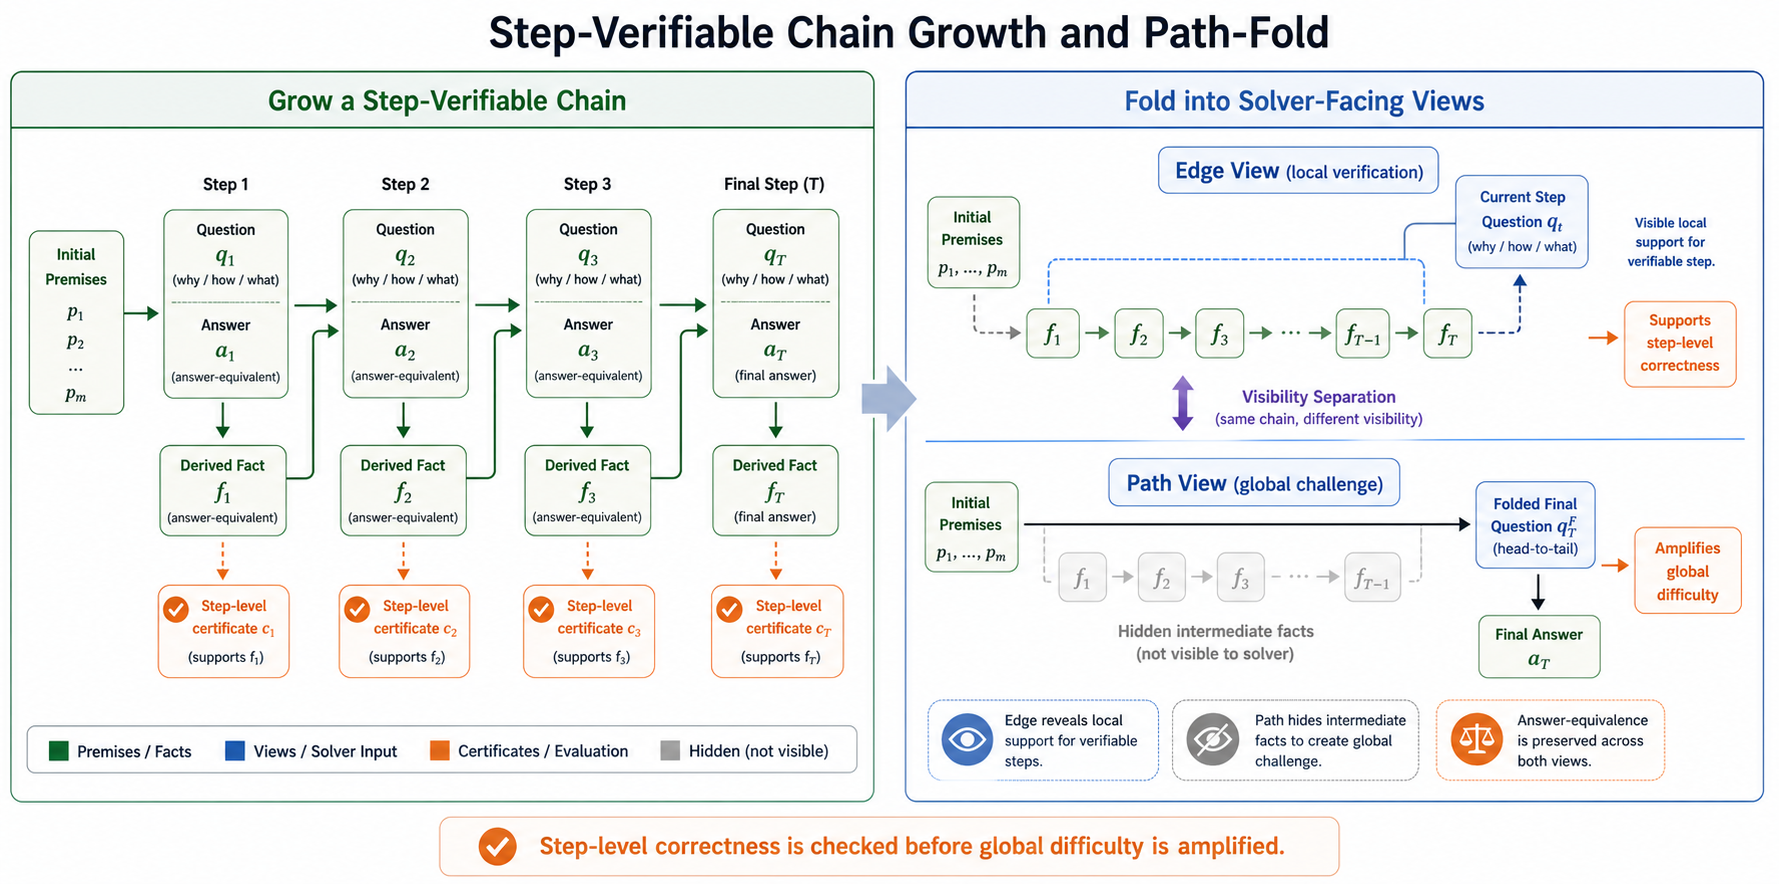
\includegraphics[width=0.94\linewidth]{figures/figure1_chain_growth_path_fold.png}
  \caption{Step-verifiable chain growth and Path-Fold. AgenQA first grows locally checkable dependency transitions, then folds intermediate facts to create a solver-facing Path View.}
  \label{fig:chain-growth}
\end{figure}

\subsection{Progressive Chain-of-KQA}

普通 QA 可以写成：
\[
x=(K,q,a),
\]
其中 $K$ 是给 solver 的已知条件，$q$ 是问题，$a$ 是目标答案。这个表示只描述最终题目，却没有说明题目是怎样被合成出来的。

AgenQA 把生成过程改成 progressive generation。每一步只在当前已知状态上扩展一个局部可检查、与答案等价的新 fact。一个步骤是一个 KQA transition：
\[
s_t=(K_t,q_t,a_t,c_t),
\]
其中 $K_t$ 是第 $t$ 步前可见的支撑信息，$q_t$ 是该步局部问题，$a_t$ 是该步得到的答案等价结论，$c_t$ 是 dependency certificate。

Certificate 记录这一答案从哪里来：
\[
c_t=(U_t,\Delta F_t,f_t),
\]
其中 $U_t$ 是该步使用的前提或先前事实，$\Delta F_t$ 是该步新产生的事实，$f_t$ 是与 $a_t$ 等价的关键事实。这些关键事实形成一条 dependency spine：
\[
K_0 \rightarrow f_1 \rightarrow f_2 \rightarrow \cdots \rightarrow f_T.
\]

这可以避免生成结果退化成一组松散相关的问题。每条 accepted chain 同时具有 locally auditable transitions 和 global dependency direction。

\subsection{Path-Fold and Solver-Facing Views}

AgenQA 将同一条 underlying chain 暴露为两种 solver-facing views。Edge View 暴露求解当前局部问题所需的支撑信息；Edge success 因此可以作为 step-level correctness 和 well-posedness 的代理信号。Path View 构造 chain-level challenge：Path-Fold 保留原始前提、定义和必要条件，但隐藏中间 key facts 和 step certificates。Solver 只能看到折叠后的最终问题，需要从可见上下文恢复通向最终答案的 latent dependency path。

一个有效 fold 至少满足：
\begin{itemize}
  \item \textbf{Answer equivalence}: 折叠后的问题仍然以尾部步骤的答案为目标答案。
  \item \textbf{Visibility separation}: 中间 key facts、step history 和内部指针不能泄露给 solver。
  \item \textbf{Path preservation}: 题目仍然可以求解，但需要重构 dependency path 或等价推理路径。
\end{itemize}

\subsection{Agentic State-Transition Harness}

\begin{figure}[H]
  \centering
  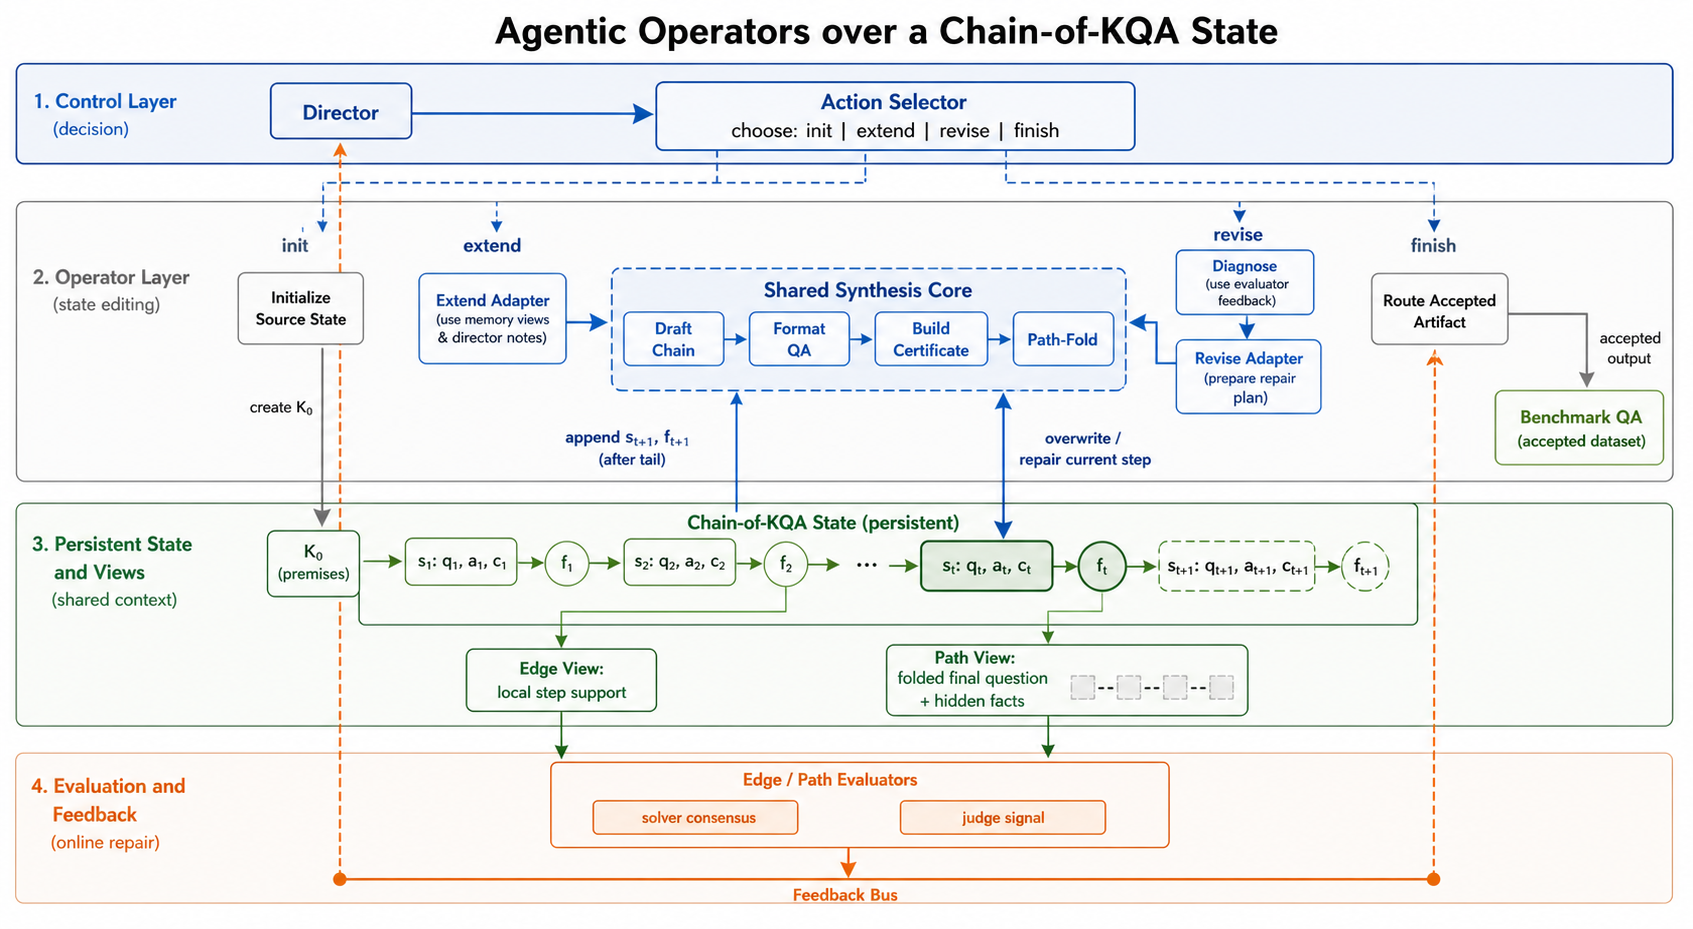
\includegraphics[width=0.94\linewidth]{figures/figure2_agentic_operators_chain_state.png}
  \caption{Agentic operators over a Chain-of-KQA state. Extension and revision reuse the same synthesis core but apply different state-edit semantics.}
  \label{fig:operators}
\end{figure}

整个 synthesis process 是作用在 progressive chain 及其 solver-facing views 上的 controlled state-transition loop：
\[
d_r = D(S_r),\qquad
S_{r+1}=O_{d_r}(S_r),\qquad
z_{r+1}=E(\Pi(S_{r+1})).
\]
其中 $S_r$ 是第 $r$ 轮 synthesis state，$D$ 是 Director controller，$d_r$ 是被选择的 operation，$O$ 是对应 Operator，$\Pi$ 构造 Edge/Path projections，$E$ 返回 solver、consensus 和 acceptance signals。

\tightparagraph{Director.} Director 负责从 available operator set 中选择下一步。它读取 progress limits、recent chain history、memory windows、available operations、question-type policy、Edge/Path solver outcomes、consensus summaries、ambiguity / contract reports 和 repair history。

\tightparagraph{Operators.} Operators 是作用在 Chain-of-KQA state 上的 structured generation procedures。Initialization 构造 starting anchor。Extension 追加新的 KQA transition。Revision 修复最新的问题 transition，同时保持该步骤在 chain 中的 intended role。在 semantic track 中，extension 和 revision 共享同一条核心 role sequence：
\[
\texttt{draft} \rightarrow \texttt{format} \rightarrow \texttt{certify} \rightarrow \texttt{fold}.
\]
二者区别在于 adapter logic 和 state-edit semantics：extension 追加新步骤，revision 覆盖或修复有问题的步骤。

\tightparagraph{Evaluator.} Evaluator 检查生成出的 Edge 和 Path views。Solvers 同时回答两种 views，consensus 聚合多个 strong-solver judgments，acceptance logic 决定当前 chain 是继续 extend、revise、accept 还是 terminate。Evaluator feedback 不是 post-hoc filter，而是 online state 的一部分，会影响后续 Director decisions。

\subsection{Scalability and Extensibility}

这个 harness 可扩展，是因为增加 chain length 或 task difficulty 不需要重新设计一个 final-question generator。每一轮都应用同一个 state-transition interface：extension 追加 transition，revision 修复问题 transition，evaluation 读取 Edge/Path projections，routing 导出 accepted states。

这个 harness 可扩展，也是因为 formal object 与 domain-specific implementations 分离。Source grounding、operator adapters、view constructors、solver ensembles 和 acceptance policies 都可以替换，同时保留 Chain-of-KQA、Edge View 和 Path View 这套接口。

\section{Evaluation Snapshot}

本节保留两张最能说明问题的表：一张展示强模型在 Path View 题目上的表现，另一张展示 Qwen 系列随模型规模变化的能力梯度。两张表共同说明：AgenQA 的 Path-Fold 不只是产生更长题面，而是在保留生成侧 dependency state 的同时，为 solver-facing benchmark 构造出可测的 difficulty 与 model-discrimination signal。

\begin{table}[H]
\centering
\small
\caption{SOTA solvers on Path View questions.}
\label{tab:sota}
\begin{tabular}{lrrrr}
\toprule
Solver & All Path View & Accuracy & Diagnostic & Diagnostic Acc. \\
\midrule
claude-sonnet-4-6 & 466 / 574 & 81.18\% & 63 / 150 & 42.00\% \\
gemini-3.1-pro-preview & 254 / 294 & 86.39\% & 47 / 78 & 60.26\% \\
glm-5 & 494 / 574 & 86.06\% & 89 / 150 & 59.33\% \\
gpt-5.4-2026-03-05 & 469 / 574 & 81.71\% & 62 / 150 & 41.33\% \\
qwen3.5-plus & 498 / 575 & 86.61\% & 90 / 150 & 60.00\% \\
\midrule
All solvers & 2181 / 2591 & 84.18\% & 351 / 678 & 51.77\% \\
\bottomrule
\end{tabular}
\end{table}

\begin{table}[H]
\centering
\small
\caption{Qwen-family scale gradient on Path View questions.}
\label{tab:qwen}
\begin{tabular}{lrrl}
\toprule
Solver & All Path View Acc. & Diagnostic Acc. & Interpretation \\
\midrule
qwen3-4b & 48.00\% & 21.55\% & lower-capacity baseline \\
qwen3-8b & 56.57\% & 34.48\% & mid-scale improvement \\
Qwen3-32B & 66.86\% & 50.00\% & larger-model improvement \\
\midrule
All solvers & 59.54\% & 38.97\% & family-level aggregate \\
\bottomrule
\end{tabular}
\end{table}

\section{Representative Path View Samples}

下面展示三道 selected Path View sample questions。它们都属于 solver-facing Path View：题面只给出最终求解所需的可见条件，中间 dependency path 被折叠，解题者需要自行恢复关键推理步骤。

\subsection{Sample 1: FedAvg 收敛界中的学习率选择}

\textbf{Subject:} Federated and Distributed Learning.

\textbf{Question.} 给定 FedAvg 设定：
\begin{itemize}
  \item 全局目标函数为
  \[
  F(w)=\sum_k \frac{n_k}{n}F_k(w),
  \]
  其中 $F_k(w)$ 是客户端 $k$ 的局部经验损失，$n_k=|D_k|$，且 $n=\sum_k n_k$。
  \item 每个客户端从 $w^t$ 出发，以常数学习率 $\eta>0$ 执行 $E>1$ 步本地 SGD，再由服务器按权重平均聚合。
  \item 客户端数据 non-IID，梯度异质性由
  \[
  G=\left(\sum_k \frac{n_k}{n}\|\nabla F_k(w)-\nabla F(w)\|^2\right)^{1/2}
  \]
  表示。全局损失满足 $L$-smoothness，一共进行 $T$ 轮通信。
\end{itemize}
要求求出使时间平均平方梯度范数上界最小的学习率 $\eta^\ast$，并给出优化后的最紧上界。

\textbf{Reference answer.}
\[
\eta^\ast=
\sqrt{\frac{2[F(w^0)-F(w^\ast)]}{L E^2G^2T}},
\qquad
\frac{1}{T}\sum_{t=0}^{T-1}\|\nabla F(w^t)\|^2
\leq
2\sqrt{\frac{2LG^2[F(w^0)-F(w^\ast)]}{T}}.
\]

\subsection{Sample 2: Pointer-Generator Coverage Loss 的梯度路径}

\textbf{Subject:} Natural Language Processing / Abstractive Summarization.

\textbf{Question.} 给定软注意力 encoder-decoder：
\[
e_{t,i}=\mathrm{score}(s_t,h_i),\qquad
a_{t,i}=\frac{\exp(e_{t,i})}{\sum_j\exp(e_{t,j})},\qquad
c_t=\sum_i a_{t,i}h_i.
\]
组合训练损失为
\[
L_{\mathrm{total}}=L_{\mathrm{NLL}}+\lambda L_{\mathrm{cov}},\qquad
\mathrm{cov}_{t,i}=\sum_{t'<t}a_{t',i},\qquad
L_{\mathrm{cov}}=\sum_t\sum_i\min(a_{t,i},\mathrm{cov}_{t,i}).
\]
要求推导 $\partial L_{\mathrm{total}}/\partial h_i$ 的单一闭式符号表达，同时捕捉 score path 与 context path。

\textbf{Reference answer.}
\[
\frac{\partial L_{\mathrm{total}}}{\partial h_i}
=
\sum_t
\left[
a_{t,i}\left(g_{t,i}-\sum_j a_{t,j}g_{t,j}\right)
\frac{\partial e_{t,i}}{\partial h_i}
+
a_{t,i}\frac{\partial L_{\mathrm{NLL}}}{\partial c_t}
\right].
\]

\subsection{Sample 3: TRADES 鲁棒训练目标的外层与内层条件}

\textbf{Subject:} Machine Learning Security / Adversarial Robustness.

\textbf{Question.} 给定参数化深度神经网络 $f_\theta$，可行扰动集合为闭 $L_p$ 球 $\{\delta:\|\delta\|_p\leq\varepsilon\}$。TRADES-style 目标为
\[
\min_{\theta}
\mathbb{E}_{(x,y)\sim\mu}
\left[
L(f_\theta(x),y)
+
\beta\max_{\|\delta\|_p\leq\varepsilon}
\mathrm{KL}\bigl(f_\theta(x)\|f_\theta(x+\delta)\bigr)
\right].
\]
要求合并推导外层 envelope-theorem gradient、$\theta^\ast$ 处外层驻点条件、内层归一化 PGD 更新规则，以及收敛时的 KKT 条件。

\textbf{Reference answer.}
\[
\nabla_\theta
\max_{\|\delta\|_p\leq\varepsilon}
\mathrm{KL}\bigl(f_\theta(x)\|f_\theta(x+\delta)\bigr)
=
\nabla_\theta
\mathrm{KL}\bigl(f_\theta(x)\|f_\theta(x+\delta^\ast(\theta))\bigr).
\]
\[
\nabla_\theta\mathbb{E}_{(x,y)\sim\mu}
\left[L(f_{\theta^\ast}(x),y)\right]
+
\beta\nabla_\theta\mathbb{E}_{(x,y)\sim\mu}
\left[
\mathrm{KL}\bigl(f_{\theta^\ast}(x)\|f_{\theta^\ast}(x+\delta^\ast(\theta^\ast))\bigr)
\right]=0.
\]
\[
\delta_{t+1}
=
\Pi_{\|\cdot\|_p\leq\varepsilon}
\left(
\delta_t+
\alpha
\frac{
\nabla_\delta\mathrm{KL}\bigl(f_\theta(x)\|f_\theta(x+\delta_t)\bigr)
}{
\left\|
\nabla_\delta\mathrm{KL}\bigl(f_\theta(x)\|f_\theta(x+\delta_t)\bigr)
\right\|_p
}
\right),
\]
\[
\nabla_\delta\mathrm{KL}\bigl(f_\theta(x)\|f_\theta(x+\delta^\ast)\bigr)
=
\lambda\nabla_\delta\|\delta^\ast\|_p,\qquad
\lambda(\|\delta^\ast\|_p-\varepsilon)=0,\qquad
\|\delta^\ast\|_p\leq\varepsilon.
\]

\section{Conclusion}

AgenQA 的核心判断是：高质量 challenging reasoning QA 不能只依赖 final question generation。难度与正确性需要被拆开处理：生成侧保留可审计、可修复的 dependency path；solver 侧通过 Path-Fold 面对被折叠后的端到端问题。这样，系统可以在每一步维持 step-level verifiability，同时让最终问题承载更长的依赖路径和更强的模型区分度。

从工程上看，Director--Operator--Evaluator loop 使 AgenQA 不只是一个 prompt pipeline，而是一个围绕显式 reasoning state 运转的 synthesis harness。它能够把 extension、revision、solver feedback、consensus、contract stabilization 和 artifact replay 组织进同一生命周期。当前展示的评测表格与样例题说明，这一设计已经能产生有可读形态、有难度信号、也能解释其难度来源的 Path View items。

\begin{thebibliography}{10}

\bibitem{fan2025megascience}
Run-Ze Fan, Zengzhi Wang, and Pengfei Liu.
\newblock MegaScience: Pushing the Frontiers of Post-Training Datasets for Science Reasoning.
\newblock arXiv:2507.16812, 2025.

\bibitem{qin2026datadarwinism}
Yiwei Qin, Zhen Huang, Tiantian Mi, Weiye Si, Chenyang Zhou, Qipeng Guo, Siyuan Feng, and Pengfei Liu.
\newblock Data Darwinism Part I: Unlocking the Value of Scientific Data for Pre-training.
\newblock arXiv:2602.07824, 2026.

\bibitem{wang2023selfinstruct}
Yizhong Wang, Yeganeh Kordi, Swaroop Mishra, Alisa Liu, Noah A. Smith, Daniel Khashabi, and Hannaneh Hajishirzi.
\newblock Self-Instruct: Aligning Language Models with Self-Generated Instructions.
\newblock arXiv:2212.10560, 2023.

\bibitem{luo2025wizardmath}
Haipeng Luo et al.
\newblock WizardMath: Empowering Mathematical Reasoning for Large Language Models via Reinforced Evol-Instruct.
\newblock arXiv:2308.09583, 2025.

\bibitem{yu2024metamath}
Longhui Yu et al.
\newblock MetaMath: Bootstrap Your Own Mathematical Questions for Large Language Models.
\newblock arXiv:2309.12284, 2024.

\bibitem{zeng2024autoevolinstruct}
Weihao Zeng, Can Xu, Yingxiu Zhao, Jian-Guang Lou, and Weizhu Chen.
\newblock Automatic Instruction Evolving for Large Language Models.
\newblock arXiv:2406.00770, 2024.

\bibitem{lu2025rhorizon}
Yi Lu et al.
\newblock R-Horizon: How Far Can Your Large Reasoning Model Really Go in Breadth and Depth?
\newblock arXiv:2510.08189, 2025.

\bibitem{xu2026compositionrl}
Xin Xu et al.
\newblock Composition-RL: Compose Your Verifiable Prompts for Reinforcement Learning of Large Language Models.
\newblock arXiv:2602.12036, 2026.

\bibitem{patel2025chase}
Arkil Patel, Siva Reddy, and Dzmitry Bahdanau.
\newblock How to Get Your LLM to Generate Challenging Problems for Evaluation.
\newblock arXiv:2502.14678, 2025.

\bibitem{butt2025benchagents}
Natasha Butt, Varun Chandrasekaran, Neel Joshi, Besmira Nushi, and Vidhisha Balachandran.
\newblock BenchAgents: Multi-Agent Systems for Structured Benchmark Creation.
\newblock arXiv:2410.22584, 2025.

\bibitem{jiao2026agenticproposing}
Zhengbo Jiao et al.
\newblock Agentic Proposing: Enhancing Large Language Model Reasoning via Compositional Skill Synthesis.
\newblock arXiv:2602.03279, 2026.

\end{thebibliography}

\end{document}
